


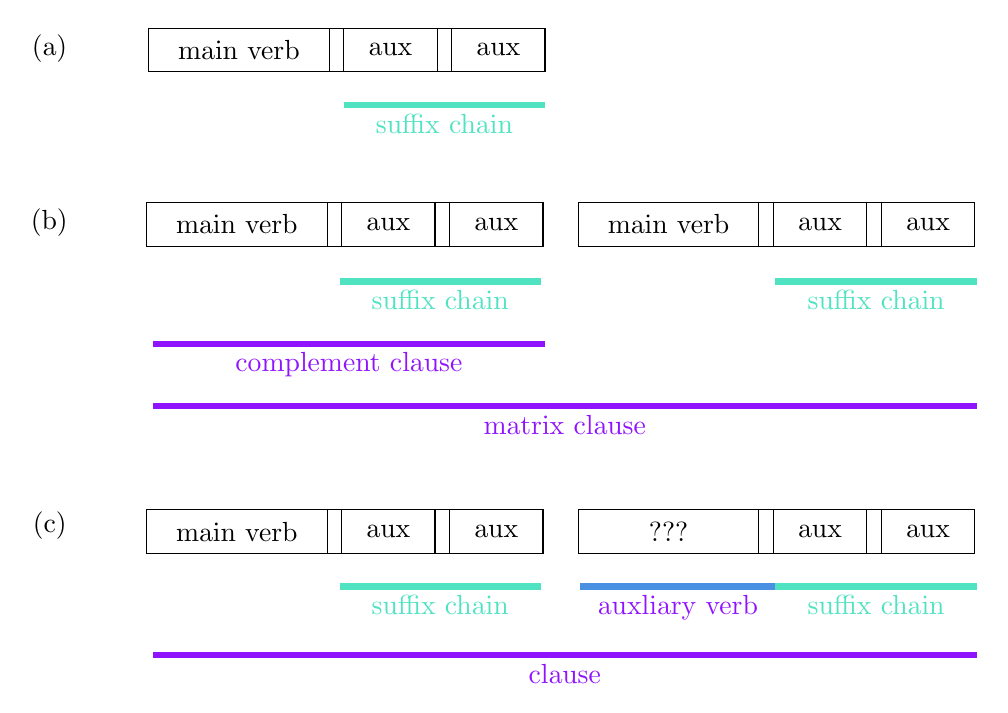
\begin{tikzpicture}[x=0.75pt,y=0.75pt,yscale=-1,xscale=1]
%uncomment if require: \path (0,507); %set diagram left start at 0, and has height of 507

%Shape: Rectangle [id:dp35161586898455655] 
\draw   (147,88.26) -- (234,88.26) -- (234,109.26) -- (147,109.26) -- cycle ;
%Shape: Rectangle [id:dp16503080821526184] 
\draw   (286,88.26) -- (241,88.26) -- (241,109.26) -- (286,109.26) -- cycle ;
%Shape: Rectangle [id:dp16255280450821386] 
\draw   (241,88.26) -- (234,88.26) -- (234,109.26) -- (241,109.26) -- cycle ;
%Shape: Rectangle [id:dp6398851060853092] 
\draw   (338,88.26) -- (293,88.26) -- (293,109.26) -- (338,109.26) -- cycle ;
%Shape: Rectangle [id:dp5923295827787749] 
\draw   (293,88.26) -- (286,88.26) -- (286,109.26) -- (293,109.26) -- cycle ;
%Straight Lines [id:da3757507657024388] 
\draw [color={rgb, 255:red, 80; green, 227; blue, 194 }  ,draw opacity=1 ][line width=2.25]    (241,125.26) -- (338,125.26) ;
%Straight Lines [id:da9972923973085535] 
\draw [color={rgb, 255:red, 80; green, 227; blue, 194 }  ,draw opacity=1 ][line width=2.25]    (239,210.26) -- (336,210.26) ;
%Straight Lines [id:da5465523467441933] 
\draw [color={rgb, 255:red, 80; green, 227; blue, 194 }  ,draw opacity=1 ][line width=2.25]    (449,210.26) -- (546,210.26) ;
%Straight Lines [id:da9103547136453445] 
\draw [color={rgb, 255:red, 144; green, 19; blue, 254 }  ,draw opacity=1 ][line width=2.25]    (149,240.26) -- (338,240.26) ;
%Straight Lines [id:da21214292532671486] 
\draw [color={rgb, 255:red, 144; green, 19; blue, 254 }  ,draw opacity=1 ][line width=2.25]    (149,270.26) -- (546,270.26) ;
%Straight Lines [id:da5062887834362] 
\draw [color={rgb, 255:red, 80; green, 227; blue, 194 }  ,draw opacity=1 ][line width=2.25]    (239,357.26) -- (336,357.26) ;
%Straight Lines [id:da23787107953327236] 
\draw [color={rgb, 255:red, 80; green, 227; blue, 194 }  ,draw opacity=1 ][line width=2.25]    (449,357.26) -- (546,357.26) ;
%Straight Lines [id:da7978827288524031] 
\draw [color={rgb, 255:red, 74; green, 144; blue, 226 }  ,draw opacity=1 ][line width=2.25]    (355,357.26) -- (449,357.26) ;
%Straight Lines [id:da7314914818351383] 
\draw [color={rgb, 255:red, 144; green, 19; blue, 254 }  ,draw opacity=1 ][line width=2.25]    (149,390.26) -- (546,390.26) ;
%Shape: Rectangle [id:dp8318830214100368] 
\draw   (146,172.26) -- (233,172.26) -- (233,193.26) -- (146,193.26) -- cycle ;
%Shape: Rectangle [id:dp9791823848488326] 
\draw   (285,172.26) -- (240,172.26) -- (240,193.26) -- (285,193.26) -- cycle ;
%Shape: Rectangle [id:dp7551650922097486] 
\draw   (240,172.26) -- (233,172.26) -- (233,193.26) -- (240,193.26) -- cycle ;
%Shape: Rectangle [id:dp9212991968444435] 
\draw   (337,172.26) -- (292,172.26) -- (292,193.26) -- (337,193.26) -- cycle ;
%Shape: Rectangle [id:dp6573200834937438] 
\draw   (292,172.26) -- (285,172.26) -- (285,193.26) -- (292,193.26) -- cycle ;
%Shape: Rectangle [id:dp8980580590320928] 
\draw   (354,172.26) -- (441,172.26) -- (441,193.26) -- (354,193.26) -- cycle ;
%Shape: Rectangle [id:dp9235071180644034] 
\draw   (493,172.26) -- (448,172.26) -- (448,193.26) -- (493,193.26) -- cycle ;
%Shape: Rectangle [id:dp0766475322070379] 
\draw   (448,172.26) -- (441,172.26) -- (441,193.26) -- (448,193.26) -- cycle ;
%Shape: Rectangle [id:dp5593612719238286] 
\draw   (545,172.26) -- (500,172.26) -- (500,193.26) -- (545,193.26) -- cycle ;
%Shape: Rectangle [id:dp9118325066537258] 
\draw   (500,172.26) -- (493,172.26) -- (493,193.26) -- (500,193.26) -- cycle ;
%Shape: Rectangle [id:dp1554128698162991] 
\draw   (146,320.26) -- (233,320.26) -- (233,341.26) -- (146,341.26) -- cycle ;
%Shape: Rectangle [id:dp1833810858919207] 
\draw   (285,320.26) -- (240,320.26) -- (240,341.26) -- (285,341.26) -- cycle ;
%Shape: Rectangle [id:dp8141735612127439] 
\draw   (240,320.26) -- (233,320.26) -- (233,341.26) -- (240,341.26) -- cycle ;
%Shape: Rectangle [id:dp26275584002034424] 
\draw   (337,320.26) -- (292,320.26) -- (292,341.26) -- (337,341.26) -- cycle ;
%Shape: Rectangle [id:dp4604350211757442] 
\draw   (292,320.26) -- (285,320.26) -- (285,341.26) -- (292,341.26) -- cycle ;
%Shape: Rectangle [id:dp8796206525042598] 
\draw   (354,320.26) -- (441,320.26) -- (441,341.26) -- (354,341.26) -- cycle ;
%Shape: Rectangle [id:dp7287630058740182] 
\draw   (493,320.26) -- (448,320.26) -- (448,341.26) -- (493,341.26) -- cycle ;
%Shape: Rectangle [id:dp4139726396039576] 
\draw   (448,320.26) -- (441,320.26) -- (441,341.26) -- (448,341.26) -- cycle ;
%Shape: Rectangle [id:dp18763826945232376] 
\draw   (545,320.26) -- (500,320.26) -- (500,341.26) -- (545,341.26) -- cycle ;
%Shape: Rectangle [id:dp936337555876763] 
\draw   (500,320.26) -- (493,320.26) -- (493,341.26) -- (500,341.26) -- cycle ;

% Text Node
\draw (190.5,98.76) node   [align=left] {main verb};
% Text Node
\draw (263.5,98.76) node   [align=left] {aux};
% Text Node
\draw (315.5,98.76) node   [align=left] {aux};
% Text Node
\draw (89.5,90) node [anchor=north west][inner sep=0.75pt]   [align=left] {(a)};
% Text Node
\draw (89,174) node [anchor=north west][inner sep=0.75pt]   [align=left] {(b)};
% Text Node
\draw (289.5,128.26) node [anchor=north] [inner sep=0.75pt]  [color={rgb, 255:red, 80; green, 227; blue, 194 }  ,opacity=1 ] [align=left] {suffix chain};
% Text Node
\draw (287.5,213.26) node [anchor=north] [inner sep=0.75pt]  [color={rgb, 255:red, 80; green, 227; blue, 194 }  ,opacity=1 ] [align=left] {suffix chain};
% Text Node
\draw (497.5,213.26) node [anchor=north] [inner sep=0.75pt]  [color={rgb, 255:red, 80; green, 227; blue, 194 }  ,opacity=1 ] [align=left] {suffix chain};
% Text Node
\draw (243.5,243.26) node [anchor=north] [inner sep=0.75pt]  [color={rgb, 255:red, 144; green, 19; blue, 254 }  ,opacity=1 ] [align=left] {complement clause};
% Text Node
\draw (347.5,273.26) node [anchor=north] [inner sep=0.75pt]  [color={rgb, 255:red, 144; green, 19; blue, 254 }  ,opacity=1 ] [align=left] {matrix clause};
% Text Node
\draw (90,320) node [anchor=north west][inner sep=0.75pt]   [align=left] {(c)};
% Text Node
\draw (287.5,360.26) node [anchor=north] [inner sep=0.75pt]  [color={rgb, 255:red, 80; green, 227; blue, 194 }  ,opacity=1 ] [align=left] {suffix chain};
% Text Node
\draw (497.5,360.26) node [anchor=north] [inner sep=0.75pt]  [color={rgb, 255:red, 80; green, 227; blue, 194 }  ,opacity=1 ] [align=left] {suffix chain};
% Text Node
\draw (402,360.26) node [anchor=north] [inner sep=0.75pt]  [color={rgb, 255:red, 144; green, 19; blue, 254 }  ,opacity=1 ] [align=left] {auxliary verb};
% Text Node
\draw (347.5,393.26) node [anchor=north] [inner sep=0.75pt]  [color={rgb, 255:red, 144; green, 19; blue, 254 }  ,opacity=1 ] [align=left] {clause};
% Text Node
\draw (189.5,182.76) node   [align=left] {main verb};
% Text Node
\draw (262.5,182.76) node   [align=left] {aux};
% Text Node
\draw (314.5,182.76) node   [align=left] {aux};
% Text Node
\draw (397.5,182.76) node   [align=left] {main verb};
% Text Node
\draw (470.5,182.76) node   [align=left] {aux};
% Text Node
\draw (522.5,182.76) node   [align=left] {aux};
% Text Node
\draw (189.5,330.76) node   [align=left] {main verb};
% Text Node
\draw (262.5,330.76) node   [align=left] {aux};
% Text Node
\draw (314.5,330.76) node   [align=left] {aux};
% Text Node
\draw (397.5,330.76) node   [align=left] {???};
% Text Node
\draw (470.5,330.76) node   [align=left] {aux};
% Text Node
\draw (522.5,330.76) node   [align=left] {aux};


\end{tikzpicture}
